\section{Compléter la figure (5 points)}

\begin{multicols}{2}
	\begin{questions}
		\question[1] Construire la figure ci-contre.
		\question[2] Construire le symétrique de ce quadrilatère par rapport à la droite $(BC)$. Noter $A'$ et $D'$ les symétriques de $A$ et $D$. Les traits de constructions doivent rester visibles.
		\question[2] On note $O$ le milieu du segment $[DD']$. Compléter la figure pour que $O$ soit le centre de symétrie de la figure. Les traits de constructions doivent rester visibles.


	\begin{center}
		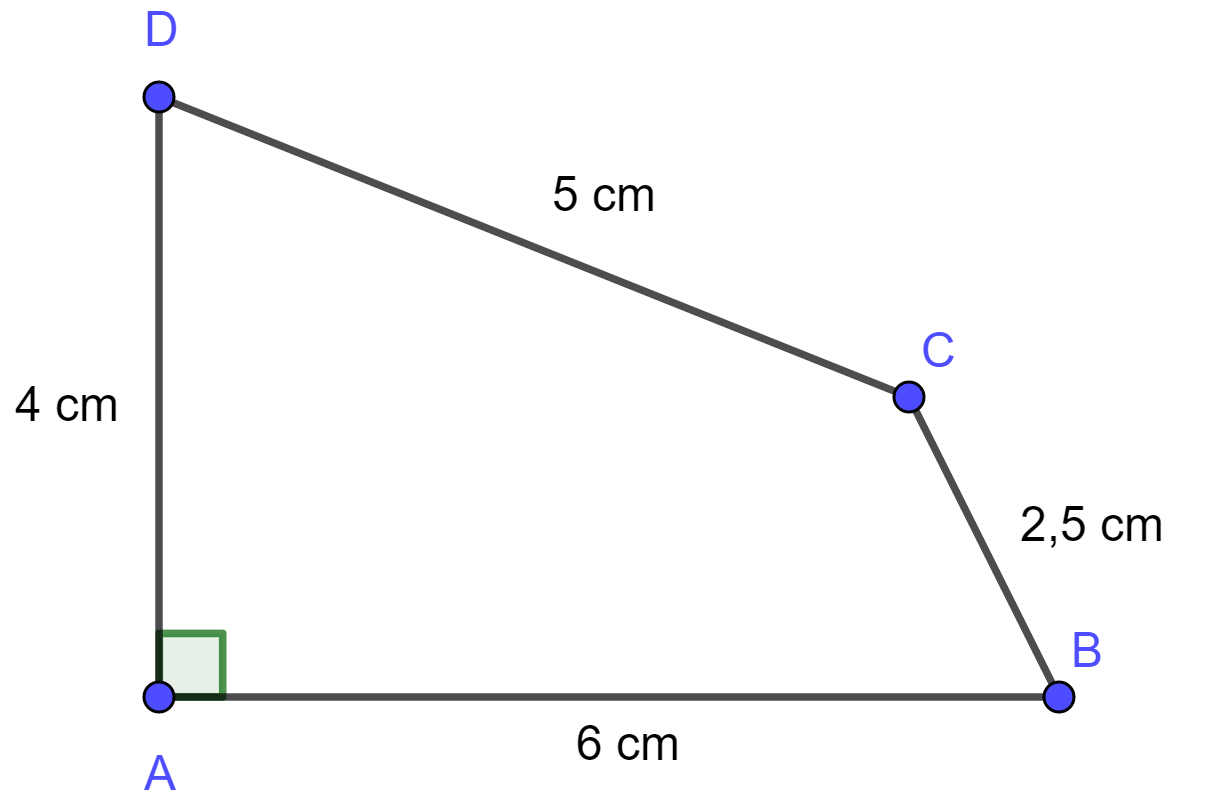
\includegraphics[scale=0.25]{img/cons}
	\end{center}

	\begin{solution}
		\begin{center}
			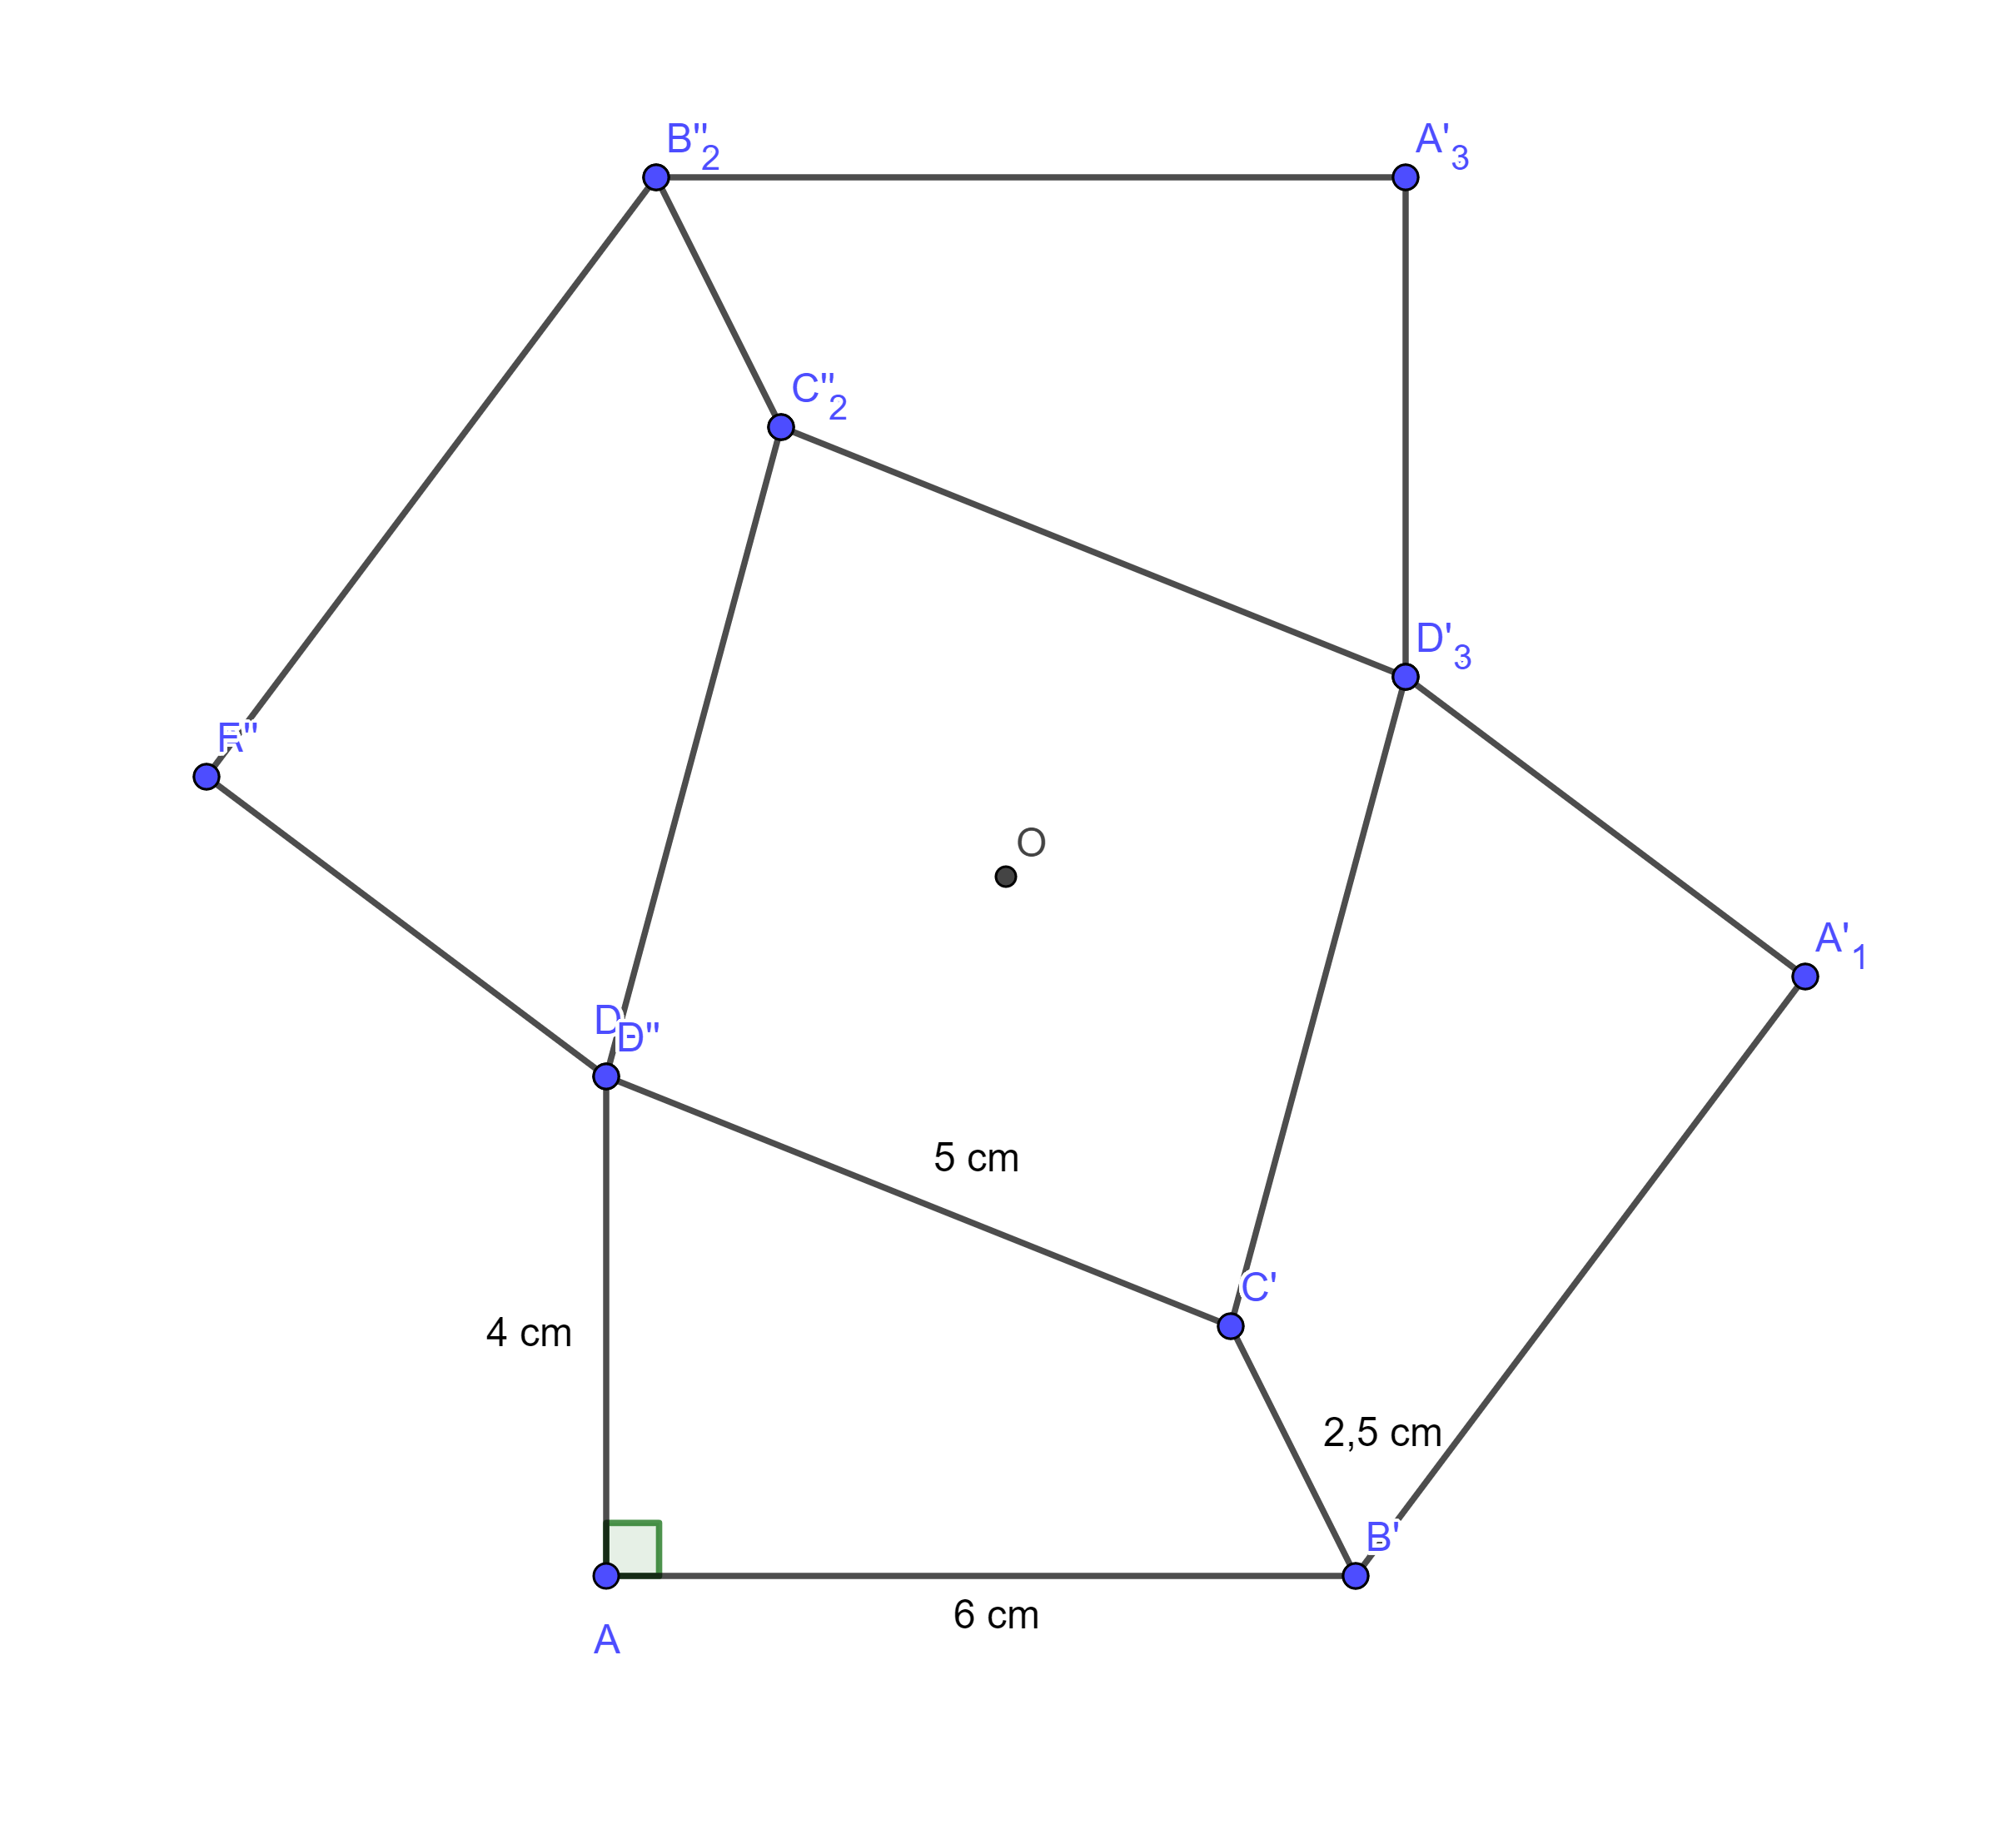
\includegraphics[scale=0.15]{img/cons_corr}
		\end{center}		
	\end{solution}


	\end{questions}
\end{multicols}

\textcolor{red}{
REMARQUE :
La construction est intéressante avec son axe de symétrie non vertical (erreur commise par beaucoup d'élèves), mais le choix du quadrilatère de départ pose problème. Les élèves commencent la figure en haut de leur copie et du coup ils n'ont pas la place pour tracer les symétriques en haut. Il vaut mieux partir du quadrilatère en haut à gauche pour éviter ce genre de problèmes.
}